\subsection{Prof. Dr. Isabel W\"{u}nsche}


\textbf{Main Research Interests}\\[-0.25cm]
\begin{enumerate}
\item[$\bullet$]	$19^{\rm th}$ and $20^{\rm th}$-Century Art and Art Theory
\item[$\bullet$]	European and American Modernism
\item[$\bullet$]	The European Avant-Garde Movements
\item[$\bullet$]	The Organic School of the Russian Avant-Garde
\item[$\bullet$]	Abstraction in Art
\item[$\bullet$]	Interrelations between Art and Science
\item[$\bullet$]	Biocentrism
\item[$\bullet$]	Synesthesia
\item[$\bullet$]	The Transatlantic Dialogue
\end{enumerate}


\vspace{0.6cm}
\textbf{Research Activities}\\[-0.25cm]

The main focus of Isabel W\"{u}nsche's work in early 2006 was the completion of her study on and the publication of the selected correspondence between Galka E. Scheyer, American representative of the Blue Four, and the Blue Four artists Lyonel Feininger, Alexej von Jawlensky, Wassily Kandinsky, and Paul Klee. Published in an English-language as well as a German-language edition by Benteli, Berne, in spring 2006, the extensively annotated correspondence focuses on the transatlantic, artistic dialogue and the introduction of European modernism to the United States. Isabel W\"{u}nsche has continued to cover the following areas: (a) organic abstraction, biocentric modernism, and the influence of the life sciences upon modernist art and design during the period 1890-1960 (various papers, major contribution to an exhibition catalogue, book chapters, preparation of an anthology with University of Pittsburgh Press); (b) ongoing work concerning the Organic School of the Russian avant-garde (various papers, book publication plans with UK publisher); (c) an extended study of the Leningrad Sterligov School that pursued abstraction in the spirit of the avant-garde during the period 1960-1990 (various papers, exhibition project at Rutgers University to be concluded in 2007). A new research project on \textit{European Modernism: Cultural Identities between National Presentation and International Orientation} was initiated with a symposium on the contribution of Russian art to European modernism in August 2006 and is currently being developed into a collaborative research project with an international team of colleagues.
\begin{figure}[ht]
  \begin{center}
    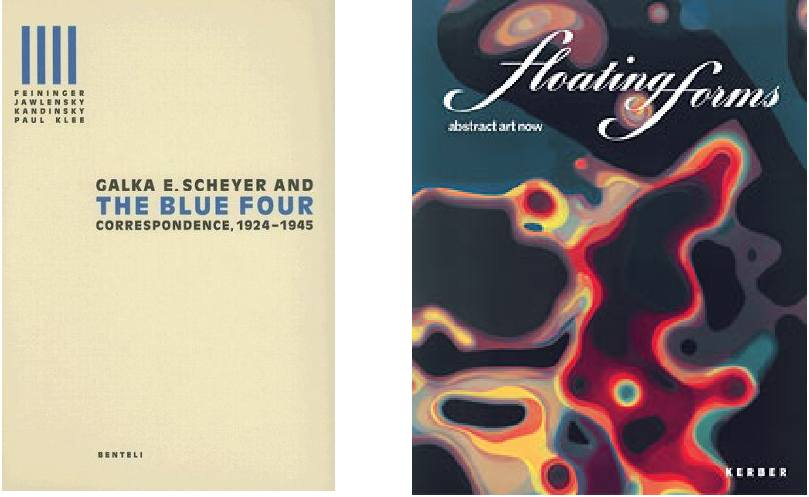
\includegraphics[width=0.85\textwidth]{./ArtLit/Wuensche.jpg}
%   \mycaption{ xxx )}\label{fig:profxxx}
   \end{center}
\end{figure}

\vspace{0.6cm}


\textbf{Funded Projects}\\[-0.25cm]
\begin{enumerate}
\item[$\bullet$]   Research Project: \textit{Der Beitrag der russischen Kunst zur europ�ischen Moderne}, funded by the Karin und Uwe Hollweg Stiftung, Bremen (research, symposium, publication)
\item[$\bullet$]   Exhibition Project: \textit{The Heritage of the Russian Avant-Garde: Vladimir Sterligov and his School}, from the Nancy and Norton Dodge Collection of Nonconformist Art from the Soviet Union at Rutgers, The State University of New Jersey, New Brunswick, funded by the Nancy and Norton Dodge Foundation
\end{enumerate}






\vspace{0.6cm}
\textbf{Organization of Scientific Conferences}\\[-0.25cm]
\begin{enumerate}
\item[$\bullet$]May 2006\newline
International University Bremen\newline
"Art and Metaphysics in the Twentieth Century and Beyond"\newline
(together with Prof. Dr. Paul Crowther \& Prof. Dr. Ursula Frohne, IUB)\newline
funded by the DFG\newline
international participants: 75
\item[$\bullet$]August 2006\newline
International University Bremen\newline
"Ferne \& N\"{a}he: Der Beitrag der russischen Kunst zur europ\"{a}ischen Moderne"\newline
(together with PD Dr. Ada Raev, Humboldt-Universit\"{a}t Berlin)\newline
funded by the Karin und Uwe Hollweg Stiftung, Bremen\newline
international participants: 50
\end{enumerate}



\vspace{0.6cm}
\textbf{Other Professional Activities}\\[-0.25cm]
\begin{enumerate}
\item[$\bullet$] Organization of a Workshop on the Nature of Abstraction in European Modernism, IUB, October 2006
\item[$\bullet$] Organization of the Conference Panel: "The Idea of Evolution in Literature and Art: How Darwin Shaped Literary Theory and Modernist Art History Writing," 20th Annual Conference of the Society of Literature, Science, and the Arts (SLSA), Dactyl Foundation, New York, November 2006
\end{enumerate}







\vspace{0.6cm}
\textbf{PhD-Students}\\[-0.25cm]

Isabelle Schwarz\newline
\textit{Archive f\"{u}r K\"{u}nstlerpublikationenen der 1960er bis 1980er Jahre}\newline
(Archives of Artists' Publications from the 1960s to the 1980s)\newline
Defense: May 2006\\[-0.15cm]

Yuliya Salauyova\newline
\textit{Walter Benjamin on Montage and Soviet Cinema: Historical and Theoretical Aspects of the "Politicization of Aesthetics"}\\[-0.15cm]

Laura Petican\newline
\textit{The Persistence of a Baroque Mentality in Arte Povera}\\[-0.15cm]

Carin Baban\newline
\textit{Image Appropriation in 20th-Century Art}\\[-0.15cm]


\vspace{0.6cm}
\textbf{Research Personnel}\\[-0.25cm]

Elina Knorpp, M.A.

